% Prof. Dr. Ausberto S. Castro Vera
% UENF - CCT - LCMAT - Curso de Ci\^{e}ncia da Computa\c{c}\~{a}o
% Campos, RJ,  2015
% Disciplina: An\'{a}lise e Projeto de Sistemas
% Aluno:


\chapter{Projeto do Sistema}

\chapter{Pontos de Vista do Sistema}

São diferentes formas e perspectivas de enxergar o sistema. O sistema pode ser visto de várias maneiras, sendo eles divididos em grupos para ter uma visão mais clara.

\section{StakHolders}

\begin{enumerate}
\item Alunos
\item Professores
\item Gerente de redes
\item Equipe de desenvolvimento
\item Funcionários
\item Governo
\item Área financeira
\item Fornecedores
\item Vestibulando 
\item Área Limpeza
\end{enumerate}

\subsection {Direto}

Entidades que fornecem informação ao sistema diretamente e recebe informações destes diretamente:

\begin{enumerate}
\item Alunos
\item Professores
\item Gerente de redes
\item Equipe de desenvolvimento
\item Funcionários

\subsection {Indireto}

O ponto de vista indireto serão as pessoas tem interesse no sistema, porém não trabalham indiretamente com o sistema:

\item Governo
\item Área financeira
\item Fornecedores
\item Vestibulando 
\item Área Limpeza
\end{enumerate}

\section {Serviços}
	\subsection {Direto:}
	\begin{enumerate}
	\item Aluno
		\begin{itemize}
		\item Matrícula
		\item Recebimento de bolsa
		\item Biblioteca
		\item Acesso à internet
		\item Úteis escolares
		\end{itemize}
		
	\item Professores
	    \begin{itemize}
		\item Nota
		\item Folha de presença
		\item Plano de aula
		\item Acesso a internet
		\item E-mail personalizado
		\end{itemize}
		
	\item Gerente de redes
		\begin{itemize}
		\item Supervisionamento a rede do servidor
		\item Relatorio das quedas
		\item Manutenção em caso de queda de rede
		\item Coordenar os estagiarios
		\item Negociações
		\end{itemize}
		
	\item Equipe de desenvolvimento
		\begin{itemize}
		\item Desenvolvimento interno do software
		\item Manutenção preventiva
		\item Correções de erro
		\item Otimização do sistema
		\item Atualização do sistema
		\end{itemize}
		
	\item Funcionários
		\begin{itemize}		
		\item Acesso ao contra-cheque
		\item financeiro
		\item Utilização de diversas ferramentas
		\item Responsabilidade
		\item Cumprimento de tarefas
		\end{itemize}
	
	\subsection {Indireto:}
	\item Governo
		\begin{itemize}
		\item Comprovante
		\item Cadastro de Instituições
		\item Elaboração de termos
		\item Emissão de documentos
		\item Validação do sistema
		\end{itemize}
			
	\item Área Financeira
		\begin{itemize}
		\item Contas a receber
		\item Contas a pagar
		\item Boletos bancários
		\item Faturas
		\item Receitas e despesas
		\end{itemize}

						
	\item Fornecedores
		\begin{itemize}
		\item Licitações
		\item Solicitação de Compras
		\item Negociação para o menor preço
		\item Data de renovação da licitação
		\item Notas fiscais
		\end{itemize}
		
	\item Vestibulando
		\begin{itemize}
		\item Informações
		\item Notas Vestibular
		\item Aprovação		
		\item Manifestação de lista de espera
		\item Exclusão
		\end{itemize}
					
	\item Área Limpeza
		\begin{itemize}
		\item Pagamentos
		\item Contra-cheque
		\item Solicitação de 2 via
		\item Estação de trabalho
		\item Férias
		\end{itemize}
		\end{enumerate}
		
\section {Hierarquia de Pontos de Vista}
	
É uma visão organizada e estruturada dos pontos de vista, no qual são mostrados todos os requisitos e pontos de vista do sistema, como mostra a Figura abaixo.
   \begin{figure}[H]
	      \centering
	       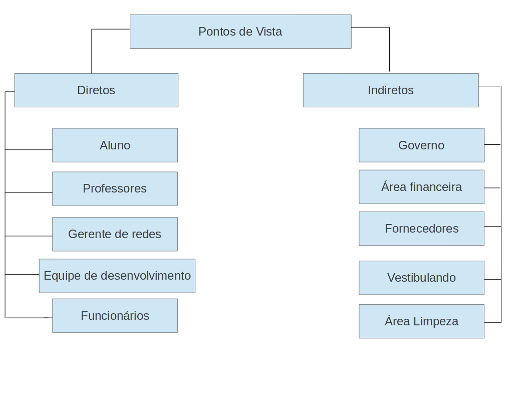
\includegraphics[width=15cm]{hierarquia2}
	       \caption{Hierarquia de Pontos de Vista}
	       \label{figRotulo}
               \end{figure}
               
               
    
 \section{Modelagem do Sistema}
 
 É um modelo abstrato do sistema representando uma visão ou perspectiva.
 Para o sistema da empresa SOFT COMPANY são construídos modelos que explicam as características
 e o comportamento de todo o sistema na base de software.
 
   \begin{figure}[H]
	      \centering
	       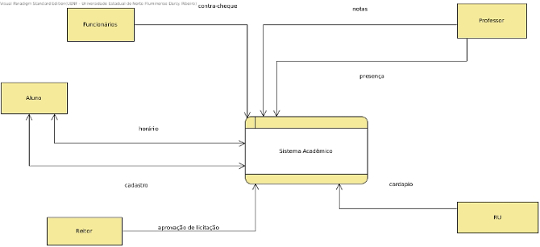
\includegraphics[width=15cm]{diagramaContexto.jpg}
	       \caption{Modelo do sistema}
	       \label{figRotulo}
               \end{figure}
               
               
\section{Entrevista}
Rodolfo da Silva,Fernando Barreto,Marco Antônio,Jennifer de Souza,José Cezar
  \subsection{Seleção de entrevistados}
  Os entrevistados serão:
Rodolfo da Silva, Aluno, será entrevistado segunda de 8:00 - 10:30
Fernando Barreto, Gerente de Banco de dados, será entrevistado segunda de 11:00 - 12:30
Marco Antônio, Economista, será entrevistado quarta de 8:30 - 10:30
Jennifer de Souza, Gerente de Relações Públicas, será entrevistada quarta de 11:00 - 12:30
José Cezar, Reitor, será entrevistado quinta de 10:00 – 12:00
Para todos os entrevistados a finalidade da entrevista será saber como o sistema tem modificado o seu trabalho diário.
 
 \subsection{Planejamento das Perguntas: 3 tipos}
 Perguntas fechadas:
 
Rodolfo da Silva

Com que frequência você utiliza o novo sistema?

Qual a redução de tempo médio que  o novo sistema trouxe?

Você gostou do designer do sistema?

Fernando Barreto
O novo sistema lhe traz transtornos com respeito a lentidão ou ter que recorrer várias vezes ao backup?
O novo sistema lhe trouxe instabilidade?
O novo sistema lhe trouxe beneficios?

Marco Antônio
O novo programa é preciso na geração de relatório de lucros?
O sistema efetua os calculos corretamente?
O plano de negócio está correto?

Jennifer de Souza
Há reclamações após a implantação do sistema?
Há comunidade se adaptou facilmente ao sistema?
Foi registrado aumento na produtividade dos funcionários?

José Cezar
Você consegue gerenciar o sistema facilmente?
O Sistema está intuitivo?
O Sistema atualiza os gráficos corretamente?



Perguntas Abertas:
Pergunta para todos os entrevistados:
Em sua opinião, o novo sistema tem facilito e agilizado seu trabalho ou estudo de forma geral?
O que você acha que poderia mudar, ser acrescentado ou retirado, no novo sistema que agilizaria e facilitaria ainda mais o seu trabalho?
Qual foi a sua experiência com o sistema?

Perguntas Analíticas:
Pergunta para todos os entrevistados:
Por que ou Como?
Obs: com relação à primeira e segunda pergunta do conjunto de perguntas abertas.
Pode ser mais específico(a)?
Obs: com relação à segunda pergunta do conjunto de perguntas abertas e caso não for bem explicado pelo entrevistado.

\subsection{Preparação para entrevista}
As perguntas serão feitas na ordem em que foram escritas, porém, irão começar pelas perguntas abertas, 
depois as perguntas analíticas, por último, as perguntas fechadas. 
Cada entrevistado possui o seu conjunto de perguntas fechadas com respostas específicas e informações
que só ele e os que trabalham na mesma área que ele possuem essas informações. 
Além de tudo, o entrevistado deverá estar trajando uma roupa social discreta para que ele e o entrevistador
possam interagir de forma que fiquem a vontade e possa ser extraída o máximo de informação do entrevistado.

\subsection{Condução da Entrevista}
 Perguntas fechadas:
Rodolfo da Silva

Com que frequência você utiliza o novo sistema?
Resposta: Todos os dias.

Qual a redução de tempo médio que  o novo sistema trouxe?
Resposta: Os alunos e funcionários estão bem mais produtivos, pois não ficam horas e horas para solicitar ou entregar documentos.

Você gostou do designer do sistema?
Resposta:Sim, bem atrativo.

Fernando Barreto

O novo sistema lhe traz transtornos com respeito a lentidão ou ter que recorrer várias vezes ao backup?
Resposta: Não, o sistema é bem eficiênte.

O novo sistema lhe trouxe instabilidade?
Resposta: Não, faz o que lhe é prometido.

O novo sistema lhe trouxe beneficios?
Resposta: Sim, produtividade.

Marco Antônio
O novo programa é preciso na geração de relatório de lucros?
Resposta: Sim, os relatórios são bem organizados.
O sistema efetua os calculos corretamente?
Resposta: Sim, não hover problema alguma desde que foi implantado.

O plano de negócio está correto?
Resposta: Sim, não há problema.

Jennifer de Souza
Há reclamações após a implantação do sistema?
Resposta: Não, a comunidade está bem satisfeita.

Há comunidade se adaptou facilmente ao sistema?
Resposta: Sim.

Foi registrado aumento na produtividade dos funcionários?
Resposta: Sim, pois os funcionários obtem qualquer documento ou dados pelo sistema.

José Cezar
Você consegue gerenciar o sistema facilmente?
Resposta: Sim, obtenho qualquer informação da universidade em 1 click.

O Sistema está intuitivo?
Resposta: Sim, ótimo gráficos e muito iterativo.

O Sistema atualiza os gráficos corretamente?
Resposta: Sim.

Perguntas Abertas:
Em sua opinião, o novo sistema tem facilito e agilizado seu trabalho/estudo de forma geral?
Respostas:

Rodolfo da Silva: Absolutamente sim, pos hoje não tenho que esperar horas e horas para ter uma informação.

Fernando Barreto: Com certeza, eficiente e seguro, definitivamente o novo sistema foi um bom investimento.

Marco Antônio: Sim e muito, com o sistema de relatórios não fico tão estressado com a possibilidade de erros de cálculos.

Jennifer de Souza: Claro que sim, só de não ter que lidar com as reclamações de antigamente já é um grande alívio.

José Cezar: Com certeza, pois hoje posso saber tudo da universidade.

O que você acha que poderia mudar, ser acrescentado ou retirado, no novo sistema que agilizaria e facilitaria ainda mais o seu trabalho?
Respostas:
Todos responderam que o sistema está ótimo ou excelente, com exceção do Fernando Barreto (Gerente de Banco de dados) que respondeu: o sistema está ótimo, porém, como todo sistema se não for feitos upgrades regulares o sistema se torna obsoleto e ineficiente, portanto, minha sugestão é que fação melhorias todo o ano para que o sistema continue como está agora, funcionando de forma rápida e eficiente.

\subsection{Acompanhamento após entrevista: relatório}

Tudo ocorreu como planejado, os entrevistados se sentiram à vontade com o tom da entrevista, responderam de maneira clara e satisfatória, ficando claro de que o sistema foi um excelente investimento e que ele deve continuar e ser melhorado, assim como foi sugerido pelo Gerente de Banco de dados Fernando Barreto, pois pode proporciona um grande aumento na eficiência da empresa e na qualidade do trabalho exercido pelos funcionários de um modo geral, desde de o gerente ao caminhoneiro.

\section{Modelagem do Sistema}
É um modelo abstrato do sistema representando uma visão ou perspectiva. Para o sistema da empresa DECKEL COMPANY são construídos modelos que explicam as características e o comportamento de todo o sistema na base de software.

\subsection{Diagrama de contexto}
Mostra como as partes interessadas e outras entidades (Figura 5.4) interagem com o sistema indicando suas entradas e saídas.
               

               \begin{figure}[H]
                 \caption{Diagrama de Contexto}
               \centering % para centralizarmos a figura
                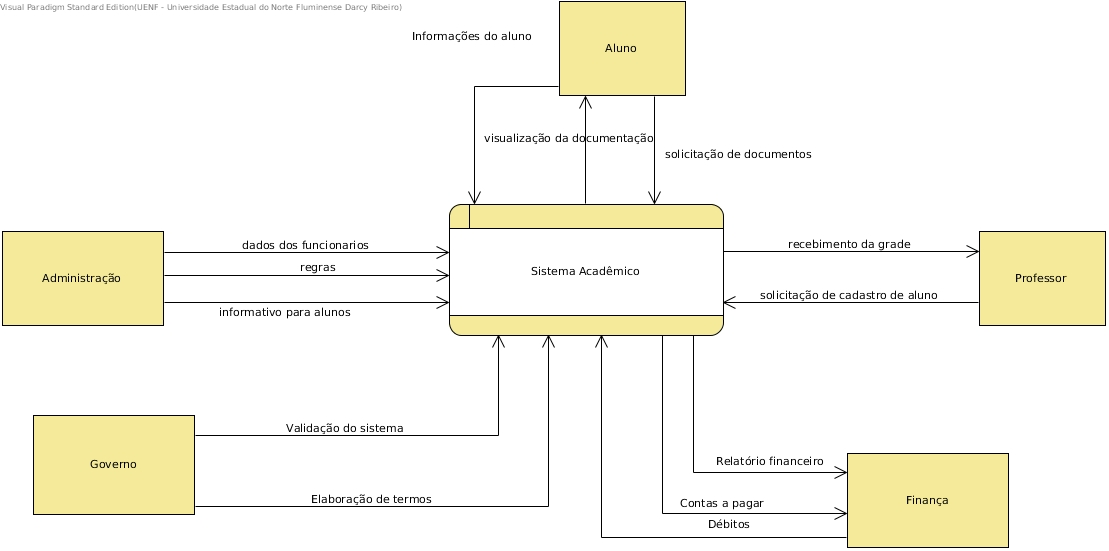
\includegraphics[width=13cm]{analisedeProjeto/DiagramadeContexto} % leia abaixo
                \label{figura:DiagramadeContexto}
                \end{figure}
                Na Fig. \ref{figura:DiagramadeContexto} , há uma visão mais geral do sistema ...
                

\subsection{Diagrama de Fluxo de Dados}
O DFD é uma técnica usada na programação estruturada de diagramação de software que possui diversos tipos de diagramas, podendo ser derivados em outros diagramas. O diagrama apresenta um modelo de organização do sistema.

                
                 
               
                  
               \begin{figure}[H]
               \caption{Nível 0}
               \centering % para centralizarmos a figura
                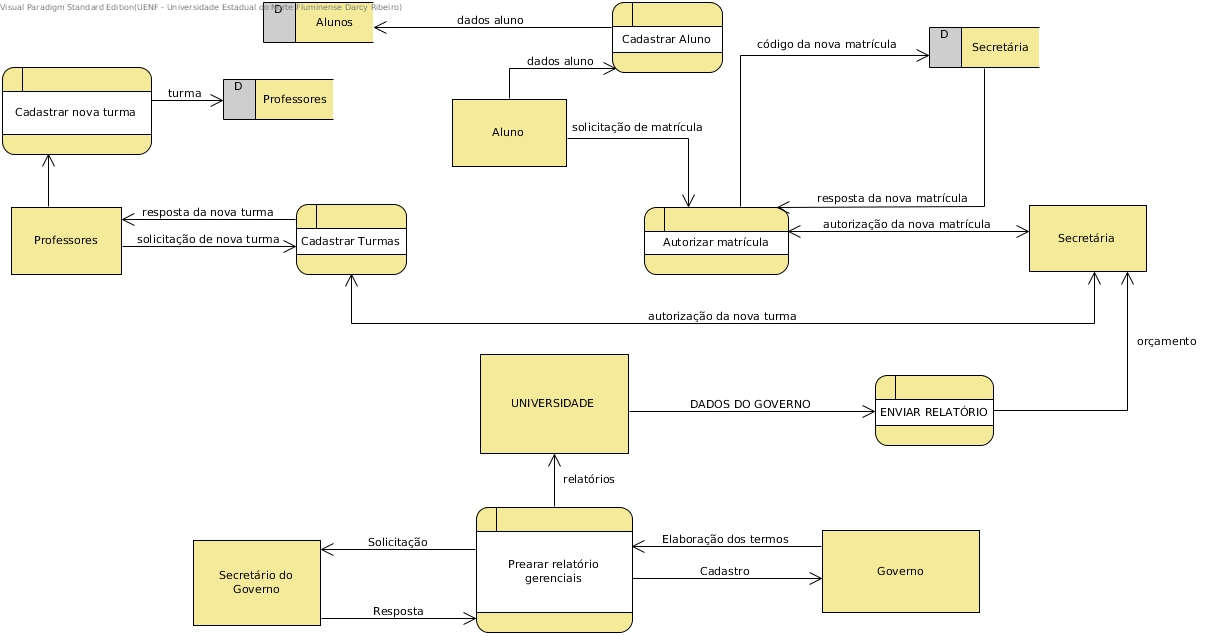
\includegraphics[width=13cm]{analisedeProjeto/DFDFisico} % leia abaixo
                \label{figura:DFDFisico}
                \end{figure}
                Na Fig. \ref{figura:DFDFisico} , há uma visão geral, porém mais detalhada do que o diagrama de contexto. ...
                  
              
                  
               \begin{figure}[H]
               \caption{Nível 1}
               \centering % para centralizarmos a figura
                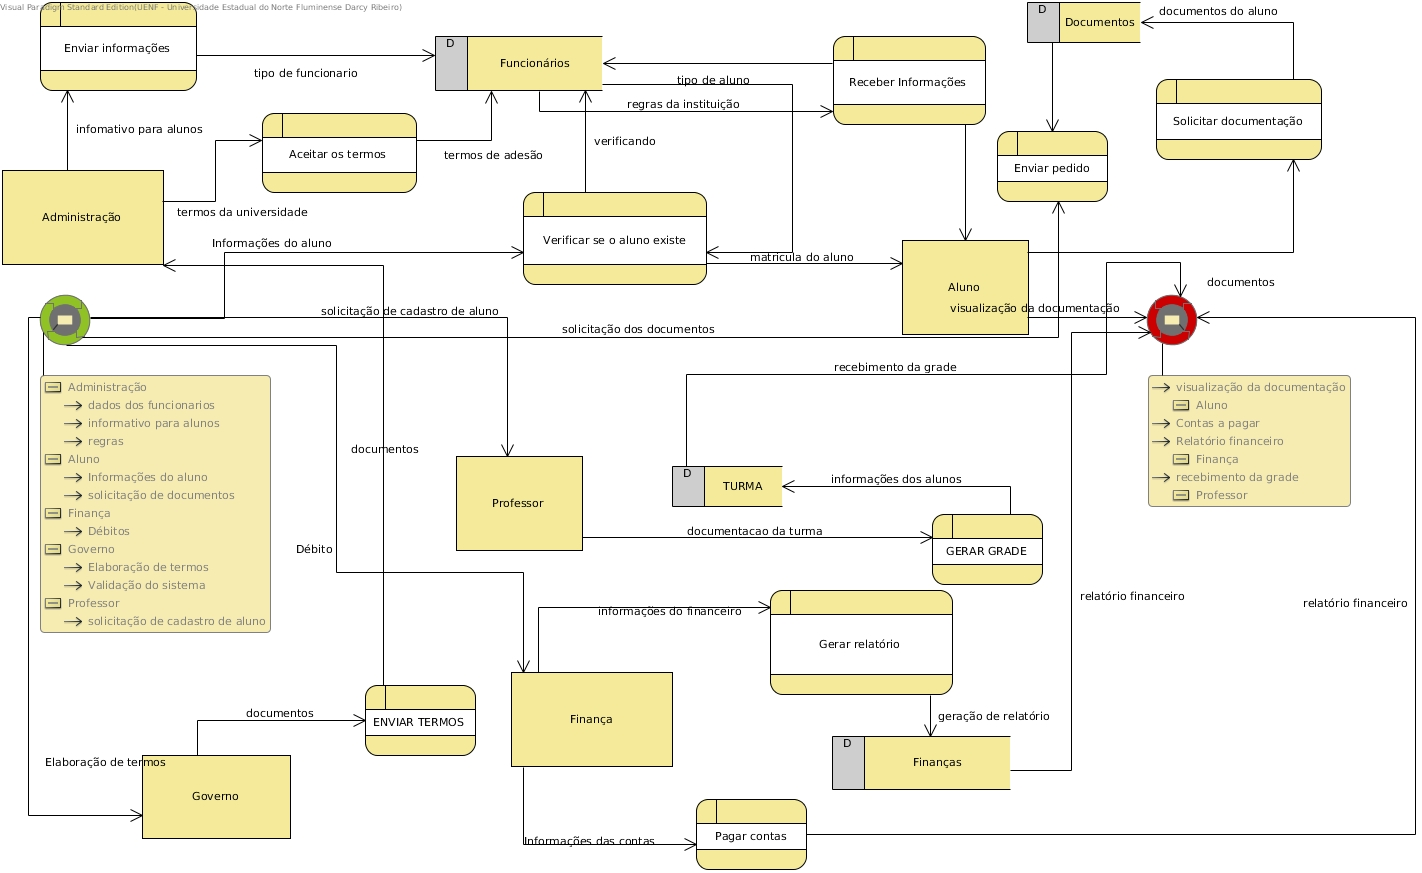
\includegraphics[width=13cm]{analisedeProjeto/Nivel1} % leia abaixo
                \label{figura:Nivel1}
                \end{figure}
                Na Fig. \ref{figura:Nivel1} , verificamos detalhes de um processo com uma entidade.
                  
                
                  
               \begin{figure}[H]
               \caption{Nível 2}
               \centering % para centralizarmos a figura
                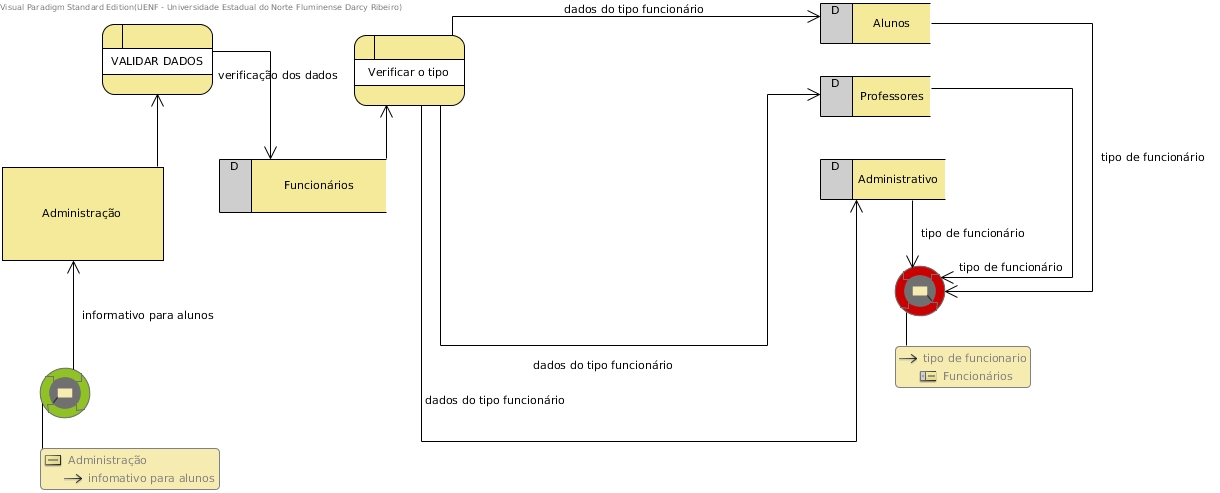
\includegraphics[width=13cm]{analisedeProjeto/Nivel2} % leia abaixo
                \label{figura:Nivel2}
                \end{figure}
                Na Fig. \ref{figura:Nivel2} , verificamos com mais riqueza de detalhes os processos, entidades e os bancos de dados.
             
                

\subsection{Entidade de Relacionamento}
É um modelo que mostra as informações que são criadas, armazenadas e usadas pelo sistema.
No diagrama (como mostra a Figura  \ref{figura:EntidadedeRelacionamento}) está representado um modelo que é usado para ajudar o desenvolvimento de um banco de dados.
 
 Um dicionário de dados (do inglês data dictionary) é uma coleção de metadados que contêm definições e representações de elementos de dados.

Dentro do contexto de SGBD, um dicionário de dados é um grupo de tabelas, habilitadas apenas para leitura ou consulta, ou seja, é uma base de dados, propriamente dita, que entre outras coisas, mantém as seguintes informações:

\begin{itemize}
 \item Definição precisa sobre elementos de dados
 \item Definição precisa sobre elementos de dados
 \item Perfis de usuários, papéis e privilégios
 \item Descrição de objetos
 \item Restrições de integridade
  \item Stored procedures (pequeno trecho de programa de computador, armazenado em um SGBD, que pode ser chamado freqüentemente por um programa principal) e gatilhos
  \item Estrutura geral da base de dados
  \item Informação de verificação
  \item Alocações de espaço
  \item Índices
\end{itemize}

Metadados, ou Metainformação, são dados sobre outros dados. Um item de um metadado pode dizer do que se trata aquele dado, geralmente uma informação inteligível por um computador. 
Os metadados facilitam o entendimento dos relacionamentos e a utilidade das informações dos dados.

 
 
               \begin{figure}[H]
                 \caption{Entidade de Relacionamento}
               \centering % para centralizarmos a figura
                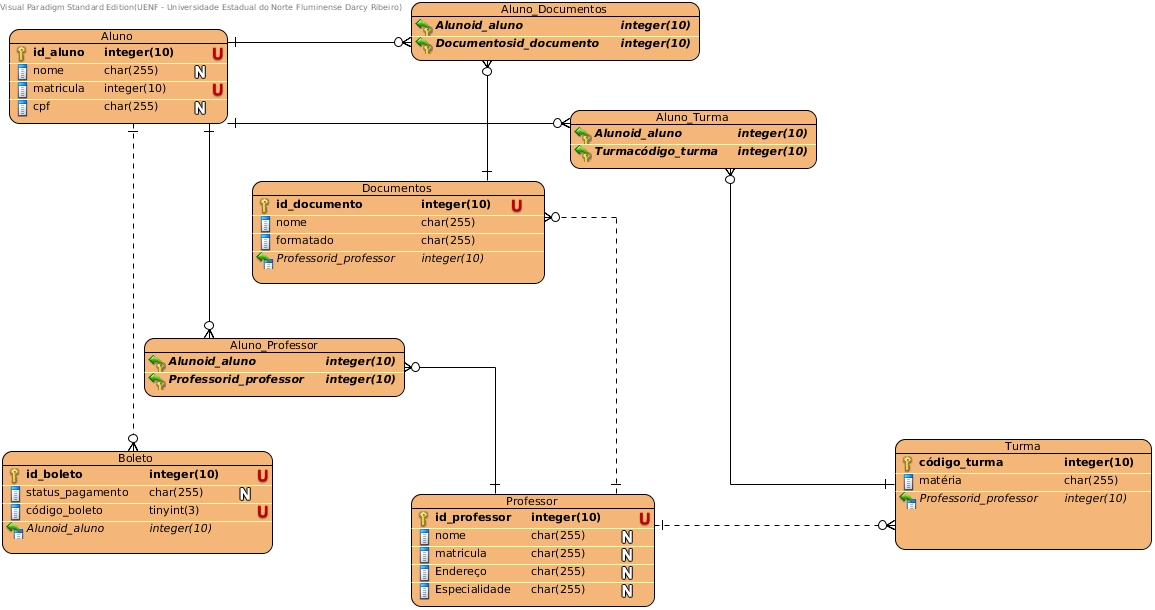
\includegraphics[width=13cm]{analisedeProjeto/SAcademicoERD} % leia abaixo
                \label{figura:EntidadedeRelacionamento}
                \end{figure}
                Na Fig. \ref{figura:EntidadedeRelacionamento} , há uma visão das tabelas do banco de dados ...

\subsection{DFD Físico}
O DFD físico representa o modo como o sistema é implementado fisicamente. Já o DFD lógico representa apenas os processos de negócio, independentemente da maneira como são implementados. A Figura \ref{figura:DFDFisico} representa a implementação de um DFD lógico para um DFD físico.



               \begin{figure}[H]
                 \caption{Diagrama De Fluxo de Dados Físico}
               \centering % para centralizarmos a figura
                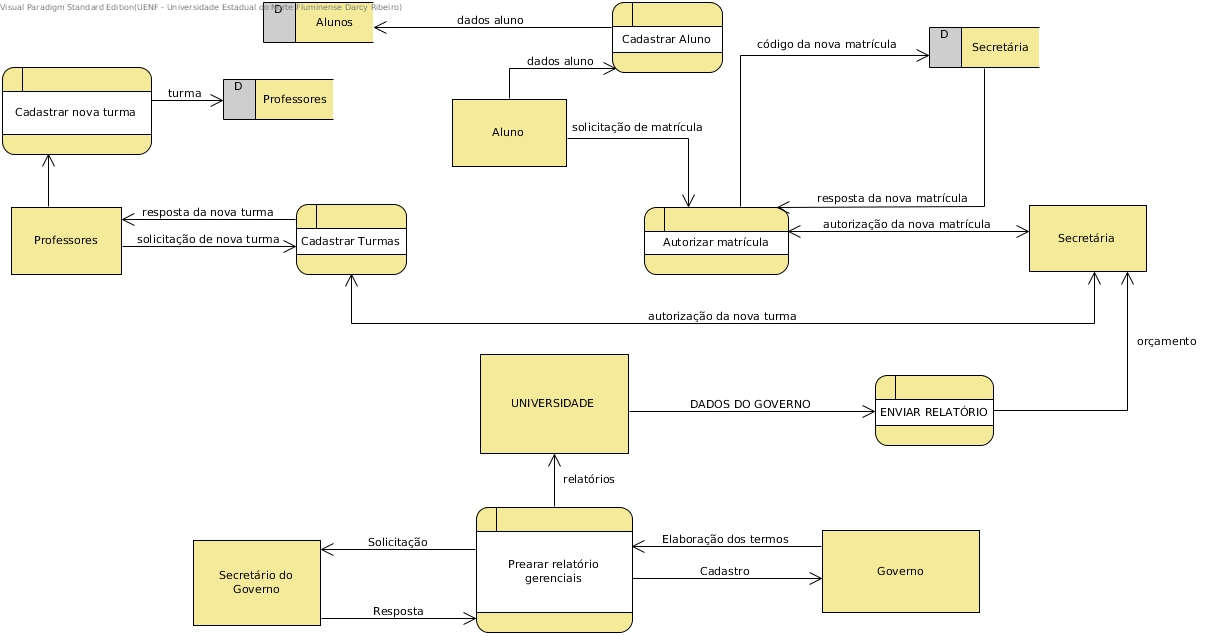
\includegraphics[width=13cm]{analisedeProjeto/DFDFisico} % leia abaixo
                \label{figura:DFDFisico}
                \end{figure}
                Na Fig. \ref{figura:DFDFisico} , há uma visão dos Diagramas De Fluxo de Dados
                
              

\subsection{ER Físico}
O ER físico apresenta mais detalhes sobre o ER (Diagrama Entidade-Relacionamento) com informações mais específicas sobre o banco de dados escolhido. Enquanto o ER lógico preocupa-se mais com os conceitos e formas de organização lógica dos dados. A Figura 7.7 representa o modelo do ER físico no Sistema de Caminhão.



       \begin{figure}[H]
                 \caption{Diagrama Entidade Relacionamento}
               \centering % para centralizarmos a figura
                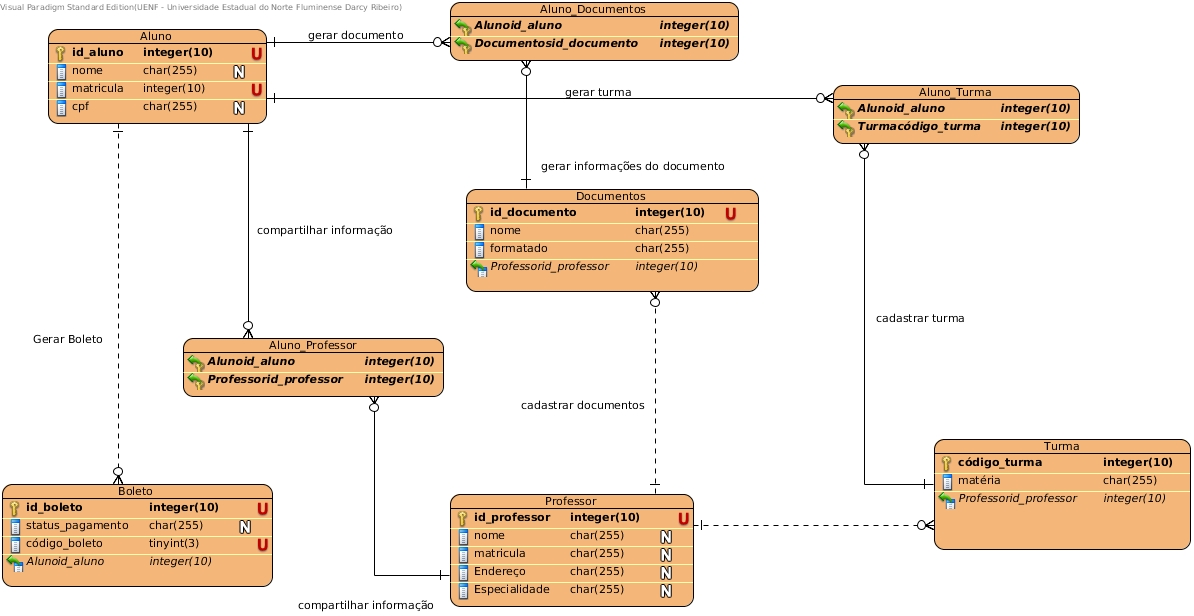
\includegraphics[width=13cm]{analisedeProjeto/ERFisico} % leia abaixo
                \label{figura:ERFisico}
                \end{figure}
                Na Fig. \ref{figura:ERFisico} , há uma visão dos Diagramas Entidade Relacionamento

\section{Estratégia do Sistema}


\subsection{Desenvolvimento Personalizado}
 O desenvolvimento personalizado é aquele no qual o desenvolvedor dentro da empresa possui o controle total sobre sua a aparência e funcionalidade. 
 O sistema permite ser flexível e criativo na maneira de solucionar problemas operacionais.
 Sistema de futebol, onde tudo deve ser personalizado e feito de forma a agregar os devidos valores para aquele seguimento.

\subsection{Sistema Pronto}
Existem muitos sistemas prontos que são comercializados para as empresas, a melhor qualidade desses sistemas são seu curto tempo de prazo, já que muitas vezes o empreendedor necessita do sistema com urgência, economizando muito tempo gasto em sua criação. O sistema a ser escolhido é sempre o que melhor atende as exigências da empresa.
Sistema de vendas online, poderá ser feito utilizando sistemas prontos, já que criar um do zero iria gerar mais custos do que do que comprar um já pronto.
\subsection{Terceirização}
 Esse serviço é utilizado na contratação de um fornecedor, desenvolvedor ou provedor de serviço externo para criar o sistema. Essas pessoas além de serem mais experientes na tecnologia, dispõem de mais recursos humanos qualificados.
 O sistema acadêmico poderia ser comprado, já que existem grandes marcas já estabelecidads.
\subsection{Estratégia do Projeto}
 Nas tabelas abaixo foram elaboradas os três tipos de Estratégias de Projeto para três situações reais diferentes, sendo que uma delas é o sistema desenvolvido neste documento (Figura 8.1, Figura 8.2 e Figura 8.3).
 
\section{Arquitetura do Sistema}
Na arquitetura são determinadas as necessidades de todas as pessoas envolvidas ou afetadas por qualquer mudança no sistema. É feita uma análise de alto nível nos requisitos do sistema, baseada nas necessidades dos usuários ou de restrições como custos e cronograma.

\subsection{Estilo de Arquitetura}
  \subsection{Arquitetura do Sistema}
  
 
  São as componentes do software, atributos externos e a comunicaç~ao com os outros softwares existentes, além de estar ligada também com a 
  arquitetura de hardware do sistema
  Abaixo são mostrados dois modelos de arquitetura de harware \ref{figura:ArquiteturaDeSoftware} e \ref{figura:modelo2Arquitetura}
  
   \textbf{Modelo 1 - Arquitetura de Sistema }
  
       \begin{figure}[H]
                 \caption{Modelo - Arquitetura de Sistema}
               \centering % para centralizarmos a figura
                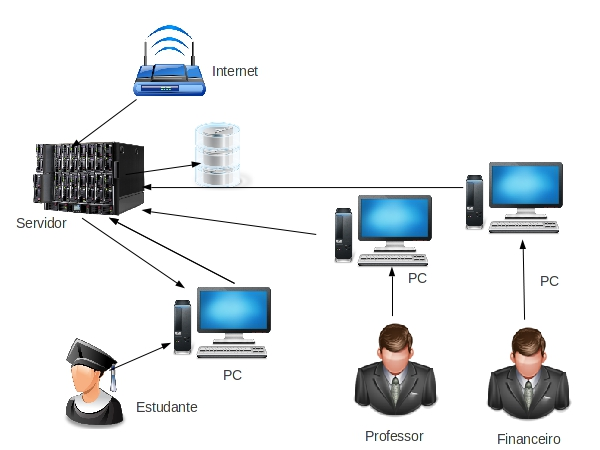
\includegraphics[width=10cm]{analisedeProjeto/ArquiteturaDeSoftware} % leia abaixo
                \label{figura:ArquiteturaDeSoftware}
                \end{figure}
                Na Fig. \ref{figura:ArquiteturaDeSoftware} , há uma da arquitetura do Sistema modelo 1
                
                
                     \textbf{Modelo 2 - Arquitetura de Sistema }  
                
                
                  \begin{figure}[H]
                 \caption{Modelo - Arquitetura de Sistema}
               \centering % para centralizarmos a figura
                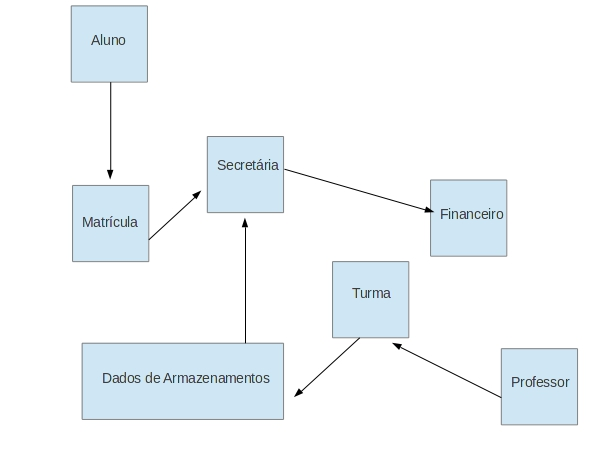
\includegraphics[width=10cm]{analisedeProjeto/modelo2Arquitetura} % leia abaixo
                \label{figura:modelo2Arquitetura}
                \end{figure}
                Na Fig. \ref{figura:modelo2Arquitetura} , há uma da arquitetura do Sistema modelo 2


                
                  \subsection{Arquitetura de Hardware}
  
 
É composta por toda a parte física que está relacionada com o sistema. Possui os componentes de hardware, suas propriedades externas e seus relacionamentos com outros hardwares já existentes
Abaixo são mostrados dois modelos de arquitetura de hardware   \ref{figura:arquiteturaDeHardware} e \ref{figura:arcloud}
  
   \textbf{Modelo 1 - Arquitetura de Hardware }
  
       \begin{figure}[H]
                 \caption{Modelo - Arquitetura de Hardware}
               \centering % para centralizarmos a figura
                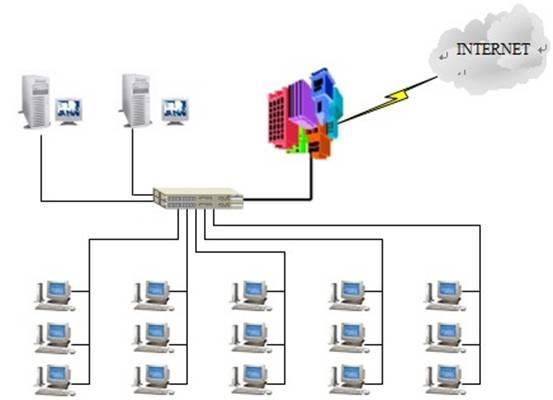
\includegraphics[width=10cm]{analisedeProjeto/arquiteturaDeHardware} % leia abaixo
                \label{figura:arquiteturaDeHardware}
                \end{figure}
                Na Fig. \ref{figura:arquiteturaDeHardware} , há uma da arquitetura de Hardware modelo 1
                
                
                     \textbf{Modelo 2 - Arquitetura de Hardware }  
                
                
                  \begin{figure}[H]
                 \caption{Modelo - Arquitetura de Hardware}
               \centering % para centralizarmos a figura
                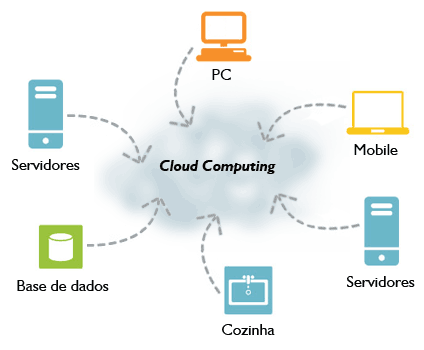
\includegraphics[width=10cm]{analisedeProjeto/arcloud} % leia abaixo
                \label{figura:arcloud}
                \end{figure}
                Na Fig. \ref{figura:arcloud} , há uma da arquitetura de Hardware modelo 2
                
                
                
                  \subsection{Arquitetura de Software}
  
 
É composta por toda a parte física que está relacionada com o sistema. Possui os componentes de hardware, suas propriedades externas e seus relacionamentos com outros hardwares já existentes
Abaixo são mostrados dois modelos de arquitetura de hardware   \ref{figura:arsoft} e \ref{figura:arSoft2}
  
   \textbf{Modelo 1 - Arquitetura de Software }
  
       \begin{figure}[H]
                 \caption{Modelo - Arquitetura de Software}
               \centering % para centralizarmos a figura
                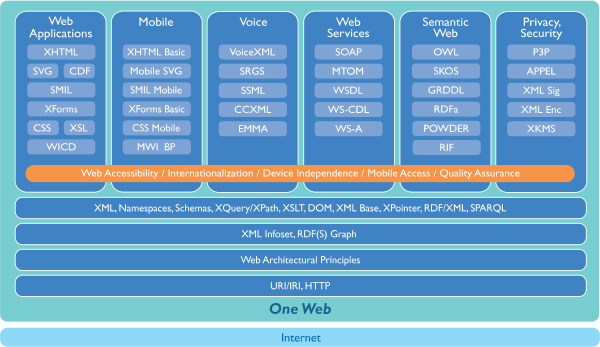
\includegraphics[width=10cm]{analisedeProjeto/arsoft} % leia abaixo
                \label{figura:arsoft}
                \end{figure}
                Na Fig. \ref{figura:arsoft} , há uma da arquitetura de Software modelo 1
                
                
                     \textbf{Modelo 2 - Arquitetura de Software }  
                
                
                  \begin{figure}[H]
                 \caption{Modelo - Arquitetura de Software}
               \centering % para centralizarmos a figura
                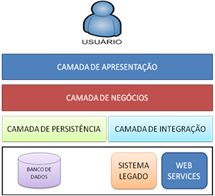
\includegraphics[width=10cm]{analisedeProjeto/arSoft2} % leia abaixo
                \label{figura:arSoft2}
                \end{figure}
                Na Fig. \ref{figura:arSoft2} , há uma da arquitetura de Software modelo 2
                
                
                
                
                
                
                
                \section{Projeto Interface}
                
                 
               \begin{figure}[H]
                 \caption{Menu}
               \centering % para centralizarmos a figura
                
\includegraphics[width=10cm]{analisedeProjeto/menu} % leia abaixo
                \label{figura:menu}
                \end{figure}
                Na Fig. \ref{figura:menu} ,  você pode visualizar o menu
                
                
                               \begin{figure}[H]
                 \caption{Menu}
               \centering % para centralizarmos a figura
                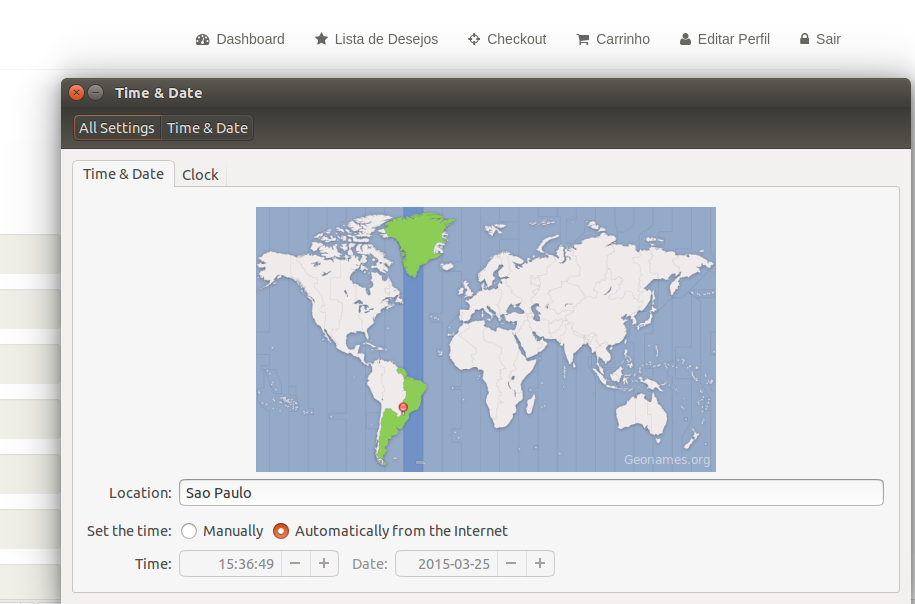
\includegraphics[width=10cm]{analisedeProjeto/menuTime} % leia abaixo
                \label{figura:menuTime}
                \end{figure}
                Na Fig. \ref{figura:menuTime} ,  você pode visualizar o menu
                


               \begin{figure}[H]
               \caption{Formulário 1}
               \centering % para centralizarmos a figura
                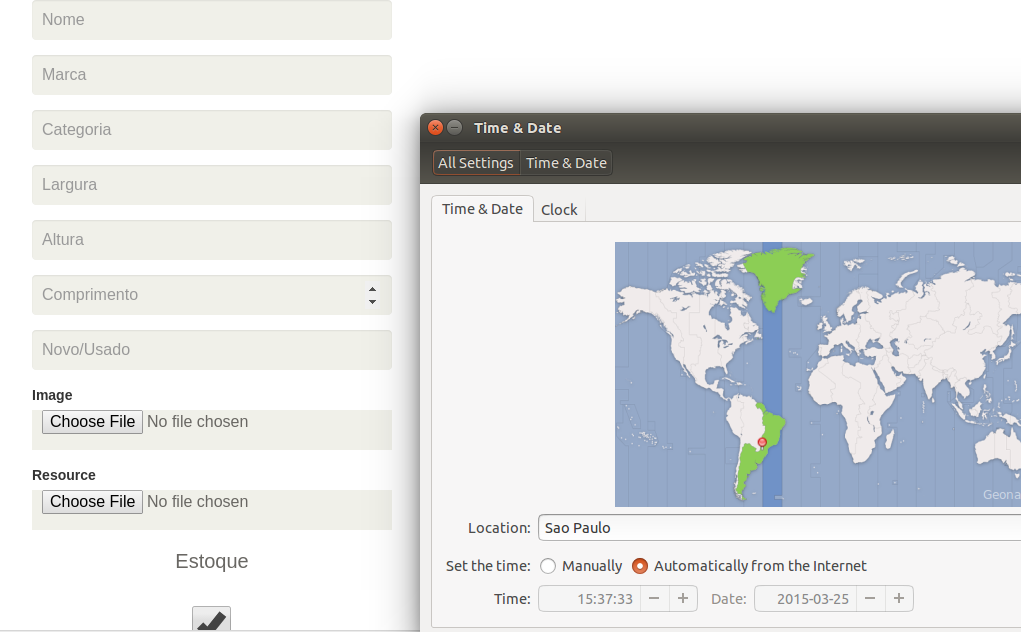
\includegraphics[width=10cm]{analisedeProjeto/form1} % leia abaixo
                \label{figura:form1}
                \end{figure}
                Na Fig. \ref{figura:form1} , você pode visualizar os formulários
                
                
                \begin{figure}[H]
                 \caption{Formulário }
               \centering % para centralizarmos a figura
                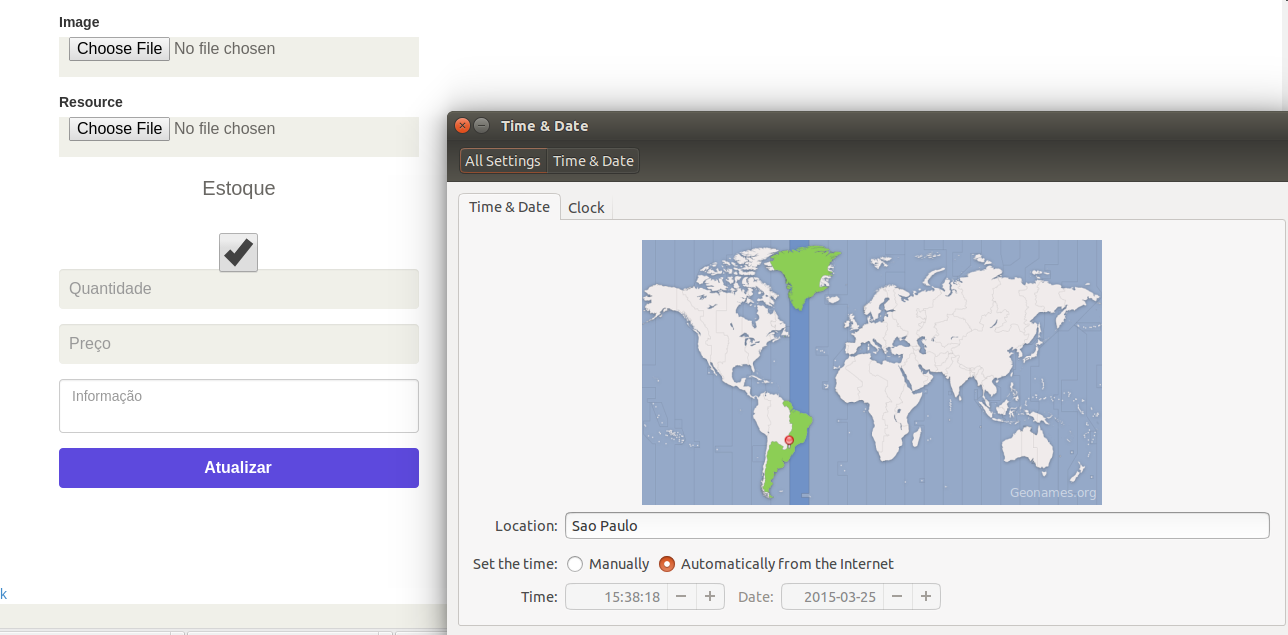
\includegraphics[width=10cm]{analisedeProjeto/form2} % leia abaixo
                \label{figura:form2}
                \end{figure}
                Na Fig. \ref{figura:form2} ,  você pode visualizar os formulários




                
\subsection{Estilos de Arquitetura}
Arquitetura do Sistema
Possui os componentes de software, suas propriedades externas e seus relacionamentos com outros softwares já existentes, além de estar ligada também com a arquitetura de hardware do sistema. Abaixo são mostrados dois modelos de arquitetura de hardware (Figura 9.3 e Figura 9.4).
Modelo 1 da Arquitetura de Software: